\documentclass[../report/report.tex]{subfiles}

\begin{document}

\subsection{Updates }
In the chapter $3$ different schedules of updates were analysed on the toy model where the parameters of the model were known a priori and no substantial discrepancies were observed in terms of the quality of approximation. 
However, in the case of the \verb|MNIST| data set estimated magnetizations allow us to perform learning of unknown parameters. Thus, in this case we combine uncertainty related to both magnetizations and parameters -- this may lead to substantial differences in performance. Figure 

\begin{figure}[!htb]
 %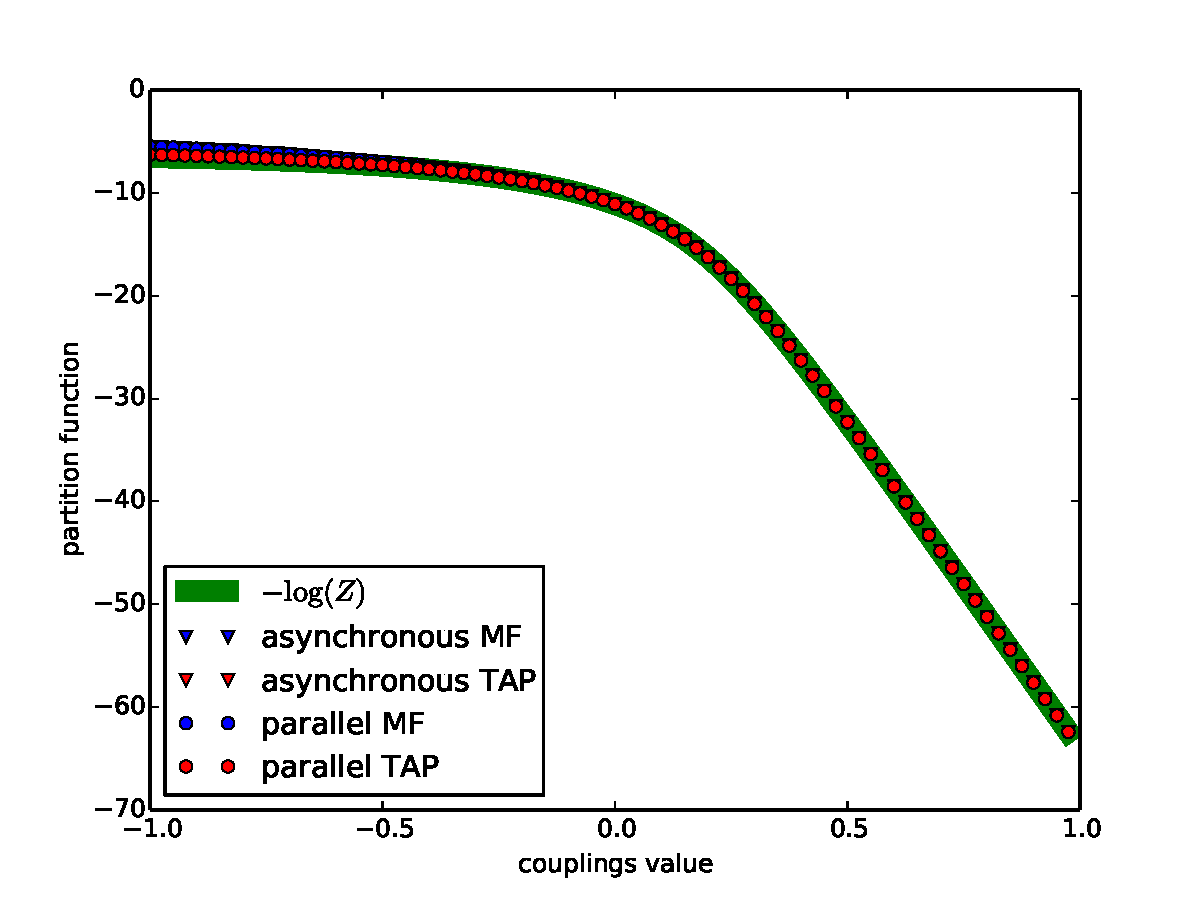
\includegraphics[width=\linewidth]{../../../Code/DRBM/toy/sameCouplingsRBMZ}
\label{fig:updatesTAP2}
  \caption[1]{updatesTAP2}
\end{figure}

\begin{figure}[!htb]
 %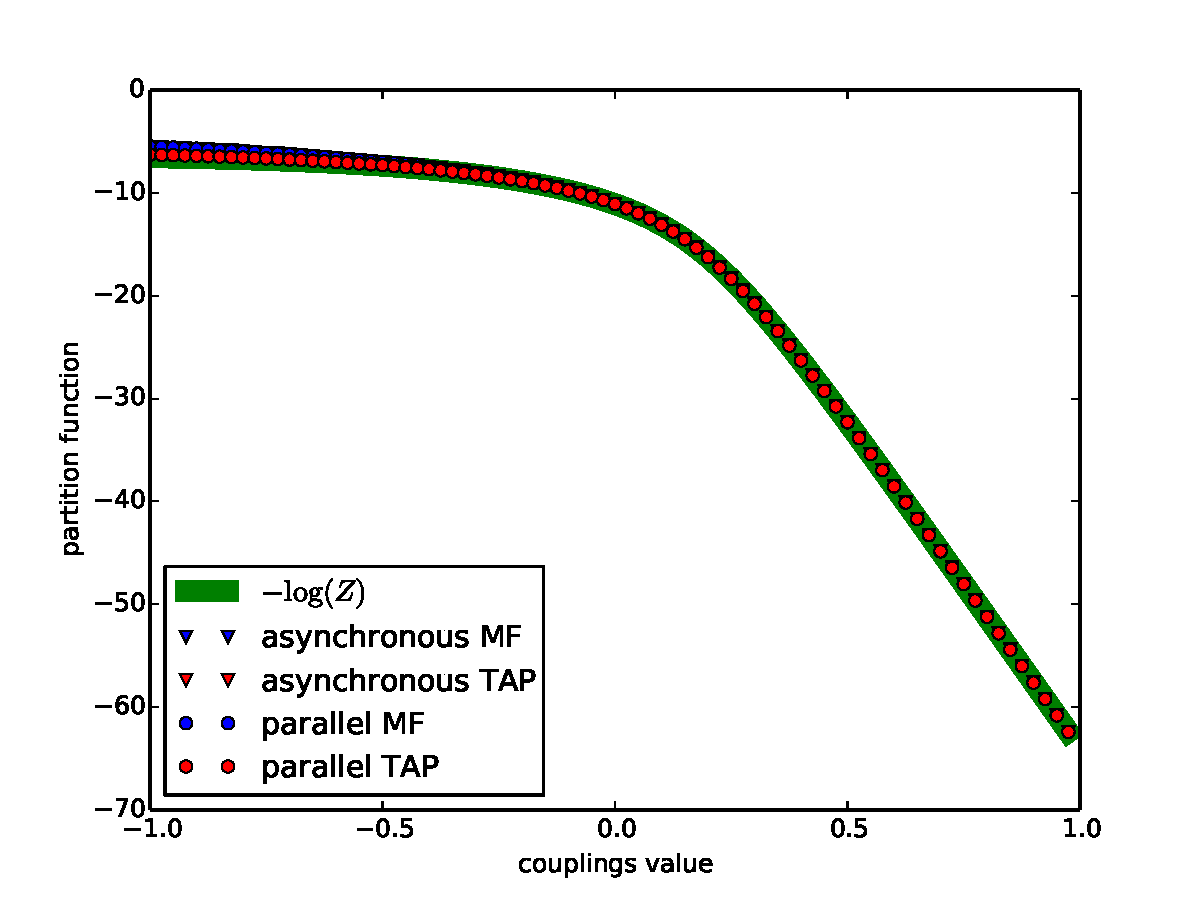
\includegraphics[width=\linewidth]{../../../Code/DRBM/toy/sameCouplingsRBMZ}
\label{fig:updatesMF}
  \caption[1]{updatesMF}
\end{figure}

\begin{figure}[!htb]
 %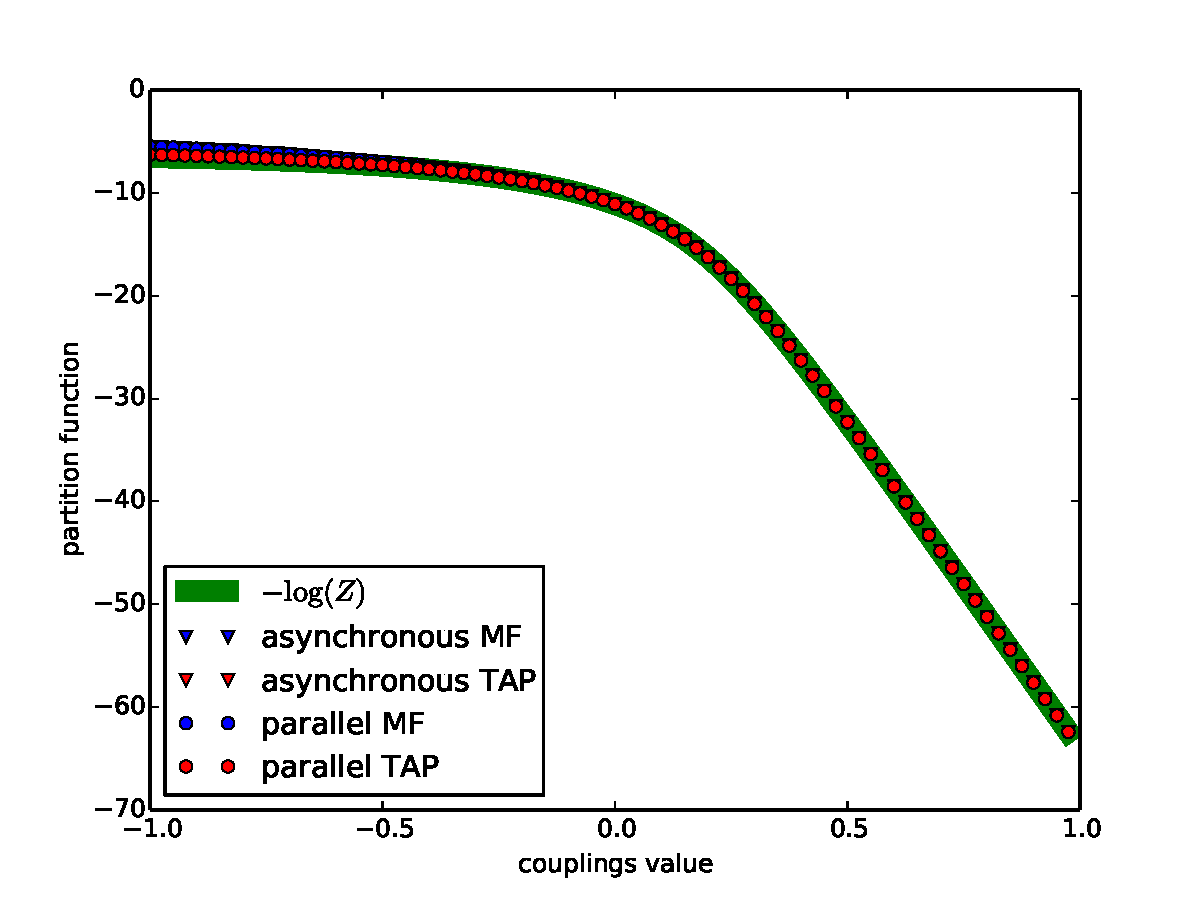
\includegraphics[width=\linewidth]{../../../Code/DRBM/toy/sameCouplingsRBMZ}
\label{fig:updatesTAP3}
  \caption[1]{updatesTAP3}
\end{figure}

\subsection{Generated samples from the models}

\subsection{AIS vs TAP}
Make several runs of AIS to get reasonable approximation!
For  all  models  we  also  used  1,000
spaced  uniformly  from  0  to  0.5,  4,000
spaced  uniformly
from 0.5 to 0.9,  and 5,000
spaced uniformly from 0.9 to 1.0,  with a total of 10,000 inter
mediate
distributions. 

\subsubsection{Annealed Importance Sampling (AIS)}

The most widely used technique is based on a very simple identity. Assume we have two distributions $p_A= \frac{1}{Z_A}p_A^*(\mathbf{x})$, $p_B= \frac{1}{Z_B}p_B^*(\mathbf{x})$ where $p^*(\dot)$ denotes unnormalized distribution and $Z_A, Z_B$ are partition functions. Assuming that a proposal $p_A$ distribution $p_A$ supports tractable sampling and tractable evaluation of both the unnormalized distribution $p_A^*(\mathbf{x})$ and the partition function $Z_A$ we can use the following relation:
\begin{align}
\begin{split}
Z_B & = \int p^*_B(\mathbf{x}) \text{d} \mathbf{x} \\ 
 &= \int \frac{p_A(\mathbf{x})}{p_A(\mathbf{x})} p^*_B(\mathbf{x}) \text{d} \mathbf{x}\\
 &=  Z_A \int \frac{ p^*_B(\mathbf{x}) }{ p^*_A(\mathbf{x}) }p_A(\mathbf{x})  \text{d} \mathbf{x} 
\end{split}
\end{align}
Sampling from the tractable distribution, we can derive Monte Carlo estimator of the ratio between partition functions:
\begin{align}
\begin{split}
\frac{Z_B}{Z_A} \approx \frac{1}{N} \sum_{i=1}^N \frac{ p^*_B(\mathbf{x}^{(i)}) }{ p^*_A(\mathbf{x}^{(i)}) } = \hat{r}_{SIS}
\label{eq:ratioSIS}
\end{split}
\end{align}
where $\mathbf{x}^{(i)}$ comes from $p_A$.
Assuming that distribution $p_A$ is close to $p_B$, the estimator from  \ref{eq:ratioSIS} called simple importance sampling proves to work well \cite{minka2005divergence}. However, in high-dimensional spaces where $p_B$ is usually multimodal as it is considered in this thesis, the variance of the estimator from \ref{eq:ratioSIS} might be very high. 

The idea presented above might be improved by following the classic approach  from probabilistic optimization i.e. simulated annealing. The idea is to introduce intermediate distributions that will allow to bridge the gap between two considered distributions $p_A$ and $p_B$ \cite{jarzynski1997nonequilibrium}, \cite{neal2001annealed}.

Consider a sequence of distributions $p_0, p_1, ..., p_M$ where $p_0 = p_A$ and $p_M = p_B$. If the intermediate distributions $p_{m}$ and $p_{m+1}$ are close enough, a simple estimator from \ref{eq:ratioSIS} can be used to estimate each ratio $\frac{Z_{m+1}}{Z_m}$. Using the the following identity: 
\begin{align}
\begin{split}
\frac{Z_M}{Z_0} = \frac{Z_1}{Z_0}\frac{Z_2}{Z_1}... \frac{Z_M}{Z_{M-1}}
\end{split}
\end{align}
those intermediate ratios are then combined to obtain the estimate of $\frac{Z_B}{Z_A}$. There is no need to compute the normalizing constants of any intermediate distributions. The intermediate distributions are chosen to suit a given problem domain. However in most cases, we are able to draw exact samples only from the first tractable distribution $p_A$. In order to sample from intermediate distribution we have be able to draw a sample $\mathbf{x}^{'}$ given $\mathbf{x}$ using Markov chain transition operator $T_m(\mathbf{x}^{'} |\mathbf{x}) $ that leaves $p_m(\mathbf{x})$ invariant, i.e.:
 \begin{align}
\begin{split}
\int T_m(\mathbf{x}^{'} |\mathbf{x}) p_m(\mathbf{x})\text{d}\mathbf{x} = p_m(\mathbf{x}^{'})
\end{split}
\end{align}
These transition operators represent the probability density of transitioning from state $\mathbf{x}$ to $\mathbf{x}^{'}$ \cite{salakhutdinov2008learning}. Having obtained the sequence of samples from the intermediate distributions we can obtain the improved estimator of the ratio between partition functions following the procedure:
\begin{algorithm}[!bthp]
\caption{Annealed Importance Sampling.}
\label{alg:vae}
\begin{algorithmic}
\State {Set $p_A$ and $p_B$ with appropriate parameters}
\For{$i \in \{1,..., N\} $} 
\State {sample $\mathbf{x}_{1}$ from $p_0 = p_A$} 
\State {sample $\mathbf{x}_{2}$ via $T_1(\mathbf{x}_{2} | \mathbf{x}_{1})$ }
\State ...
\State {sample $\mathbf{x}_{M}$ via $T_M(\mathbf{x}_{M} | \mathbf{x}_{M-1})$}
\State $r^{(i)}_{AIS} = \frac{ p^*_1(\mathbf{x}_1) }{ p^*_0(\mathbf{x}_1) }\frac{ p^*_2(\mathbf{x}_2) }{ p^*_1(\mathbf{x}_2) } ... \frac{ p^*_M(\mathbf{x}_M) }{ p^*_{M-1}
(\mathbf{x}_M) }$
\EndFor
  \State {$\hat{r}_{AIS} = \frac{1}{N} \sum_{i=1}^N \hat{r}^{(i)}_{AIS}$}
\end{algorithmic}
\end{algorithm}

It was proven that the variance of $\hat{r}_{AIS}$ will be proportional to $1 / MN$ assuming we used sufficiently large numbers of intermediate distributions $M$ \cite{neal2001annealed}. Moreover, the estimate of $Z_M / Z_0$ will be unbiased if each ratio is estimated using $N=1$ and a sample $\mathbf{x}^{m}$ is obtained using Markov chain starting at previous sample. This follows from the observation that the AIS procedure is an simple importance sampling defined on an extended state space $\mathcal{X} = (\mathbf{x}_1, \mathbf{x}_2, ..., \mathbf{x}_M)$.

The procedure described above can be adapted to the RBM case -- assume that we have estimated parameters $\mathbf{\theta}_B$ of the model that we want to evaluate. Following \cite{salakhutdinov2008quantitative} as a tractable starting distribution $p_A$ we can use "clamped" restricted Boltzmann machine where there is no hidden layer. The sequence of intermediate distribution is then defined as:
 \begin{align}
\begin{split}
p_m(\mathbf{v}) = \frac{1}{Z_m}p^*_m(\mathbf{v}) = \frac{1}{Z_m}\sum_\mathbf{h} \exp(-E_m(\mathbf{v, h}))
\end{split}
\end{align}
where $m = 0, ..., M$, $\mathbf{h} = \mathbf{h_B}$, and the energy function has the form:
 \begin{align}
\begin{split}
E_m(\mathbf{v,h}) = (1- \beta_m) E(\mathbf{v} ;\theta_A) + \beta_m E(\mathbf{v, h} ;\theta_B) 
\end{split}
\end{align}
where $\beta_m \in [0, 1]$ with $\beta_m = 0$ yielding $p_A$ and $\beta_m = 1$ giving $p_B$. Annealing slowly the "temperature" from infinity to zero we  gradually moves from the state space of proposal distribution to the space defined by the untractable distribution. Following the approach from \ref{eq:TODOderivepropertiesofRBM} we can obtain transition operators for hidden and visible variables:
 \begin{align}
\begin{split}
p(h^A | \mathbf{v}) & = \sigma ((1 - \beta) NONE \\
p(h^B) & =
\end{split}
\end{align}

\begin{algorithm}[!bthp]
\caption{Appendix -- Implementation for BM and RBM.}
\label{alg:vae}
\begin{algorithmic}
\State $\theta, \phi \gets .$
\While {$\textrm{not converged in } \theta, \phi$}
  \State {Pick subset of size $\mathbf{x}_{1:M}$ from the full dataset uniformly at random.}
  \State {Compute $g \gets \nabla_{\theta, \phi} {\tilde{\mathcal{L}}^B}{\theta, \phi; \mathbf{x}_{1:M}, \epsilon_{1:M}}$}
\EndWhile
\end{algorithmic}
\end{algorithm}

\subsubsection{Comparison}
Two models were estimated with $5$ of magnetizations to compare the quality of the approximation of the variational free energy. Figure \ref{fig:AISTAP2} presents the estimates of \ref{eq:freeEnergy} for the \verb|TAP2| and \verb|TAP3| models along with AIS estimates for different numbers of runs.

\begin{figure}[!htb]
 %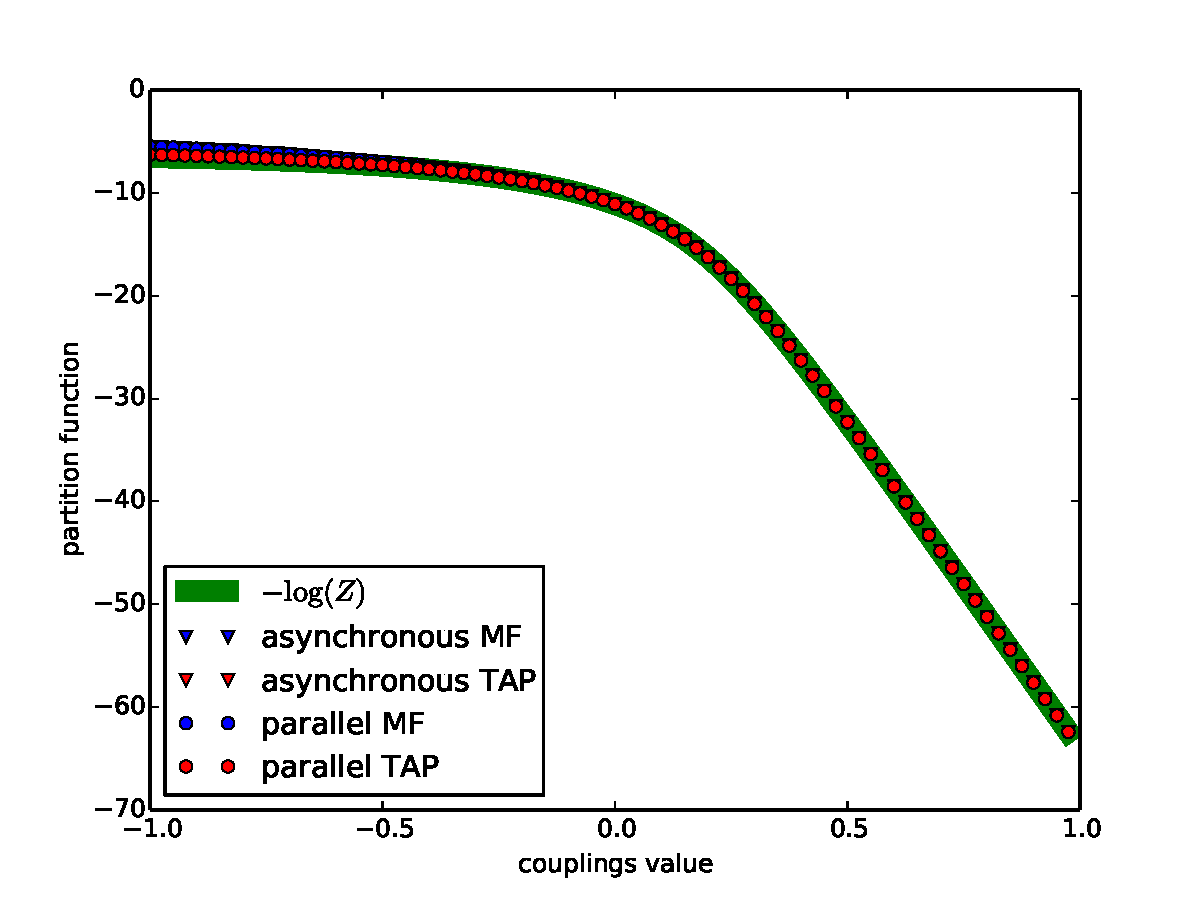
\includegraphics[width=\linewidth]{../../../Code/DRBM/toy/sameCouplingsRBMZ}
\label{fig:AISTAP2}
  \caption[1]{AIS for TAP2 and TAP3}
\end{figure}
TAP2, TAP3
3 or 10 steps of magnetization!

\subsection{Deep RBM}
\subsubsection{Unsupervised Pre-training of Neural Networks}
add Erham here

renormalization group
erham
In the previous chapter it was argued that the unsupervised pre-training . 
science
Deep learning methods

\subsubsection{Deep belief nets}
Following the approach from 
The breakthrough to effective training strategies for deep architectures came in 2006 with the CD algorithm for training
Deep Belief networks (DBN) \cite{hinton2006reducing}. DBNs are generative graphical models with many hidden layers of hidden
causal variables which joint distribution has the following form:
\begin{align}
\begin{split}
p(\mathbf{x}, \mathbf{h}^1, \mathbf{h}^2,..., \mathbf{h}^l) = p(\mathbf{x}| \mathbf{h}^1)P(\mathbf{h}^1|\mathbf{h}^2)...
P(\mathbf{h}^{l-2}|\mathbf{h}^{l-1})P(\mathbf{h}^{l-1}|\mathbf{h}^{l}).
\end{split}
\end{align}
It was shown that adding an extra layers always improve a lower bound \ref{eq:lowerboundhowtodefine} on the training data
if the number of feature detectors per layer is sufficiently large and the weights are initialized correctly. It was empirically
proven that Figure \ref{fig:DBN} depicts the exemplary deep belief network.
DBNs can be formed using a greedy layer-wise unsupervised training of stacked RBMs -- algorithm \ref{alg:DBN} presents how the process
folows:
http://www.yann-ollivier.org/rech/publs/deeptrain.pdf - show the picture 
\begin{algorithm}[!bthp]
\caption{Learning Deep Belief Nets.}
\label{alg:DBN}
\begin{algorithmic}
\State {Train the first layer as an RBM, learning $P(\mathbf{x = h^{0}, h^1}$}
\For{$l \in \{2,..., L\} $} 
\State {Pass the mean activities $\mathbf{x}^l = P(\mathbf{h^{l}| \mathbf{h^{l-1}} }$ which become a representation of the input at the layer $l$.}
\State {Train the $l$-th layer treating it as an RBM with $\mathbf{x}^l$ as an input. }
\EndFor
\end{algorithmic}
\end{algorithm}
This simple and intuitive algorithm proved to be an effective way of pretraining deep structures which laid the foundations
of the resurgence of deep neural networks. Originally, the building blocks are trained following constrastive divergence 
procedure.  However, the positive results obtained using extended mean-field approximation 
suggests that we may 
follow this procedure 

\cite{montufar2010refinements}
\begin{theorem} [Guido-Ay, 2010] Let $n = \frac{2^b}{2} + b$, $b \in \mathbb{N}$, $b \geqslant 1$. A DBN containing $\frac{2^n}{2(n-b)}$ hidden layers of size $n$ is a universal approximator of distributions on $\{0,1 \}^n$.
\end{theorem}

 The guarantee that we improve the bound is no longer valid if the size of subsequent hidden layers is not large enough
 however it was empiracally proven that such approach still can learn an effective generative model. After pretraining multiple layers of feature detectors, the model can be ``unfolded'' to form an autoencoder structures 
where the decoder network uses transposed weigths of the encoder network. At this stage, such network might be considered
as feed forward deep neural architecture and might be used as a starting point for supervised fine-tuning with respect to any
training criterion that depends on the learnt representation \ref{bengio2007greedy}.
 
 \def\layersep{2.5cm}
\begin{figure}[!h]
\begin{center}
\begin{tikzpicture}[shorten >=1pt,->,draw=black!50, node distance=\layersep]
    \tikzstyle{every pin edge}=[<-,shorten <=1pt]
    \tikzstyle{neuron}=[circle,fill=black!25,minimum size=17pt,inner sep=0pt]
    \tikzstyle{input neuron}=[neuron, fill=blue!50];
    \tikzstyle{output neuron}=[neuron, fill=red!50];
    \tikzstyle{hidden neuron}=[neuron, fill=blue!50];
     \tikzstyle{shidden neuron}=[neuron, fill=blue!50];
          \tikzstyle{thidden neuron}=[neuron, fill=black!50];
    \tikzstyle{annot} = [text width=4em, text centered]

    % Draw the input layer nodes
    \foreach \name / \y in {1,...,3}
    % This is the same as writing \foreach \name / \y in {1/1,2/2,3/3,4/4}       
     \node[input neuron, pin=left:Input \#\y] (I-\name) at (0,-\y) {};

    % Draw the hidden layer nodes
    \foreach \name / \y in {1,...,4}
        \path[yshift=0.5cm]
            node[hidden neuron] (H-\name) at (\layersep,-\y cm) {};

    % Draw the SECOND hidden layer nodes
    \foreach \name / \y in {1,...,4}
        \path[yshift=0.5cm]
            node[shidden neuron] (S-\name) at (2*\layersep,-\y cm) {};
            
            
    % Draw the THIRD hidden layer nodes
    \foreach \name / \y in {1,...,4}
        \path[yshift=0.5cm]
            node[thidden neuron] (T-\name) at (3*\layersep,-\y cm) {};

%    % Draw the output layer node
%    \node[output neuron,pin={[pin edge={->}]right:Output}, right of=S-3] (O) {};

    % Connect every node in the input layer with every node in the
    % hidden layer.
    \foreach \source in {1,...,3}
        \foreach \dest in {1,...,4}
            \path (I-\source) edge (H-\dest);
            
% Connect every node in the hidden layer with every node in the
    % SECOND hidden layer.
    \foreach \source in {1,...,4}
        \foreach \dest in {1,...,4}
            \path (H-\source) edge (S-\dest);

% Connect every node in the hidden layer with every node in the
    % SECOND hidden layer.
    \foreach \source in {1,...,4}
        \foreach \dest in {1,...,4}
            \path (S-\source) edge (T-\dest);
            
%    % Connect every node in the hidden layer with the output layer
%    \foreach \source in {1,...,5}
%        \path (H-\source) edge (O);

    % Annotate the layers
    \node[annot,above of=H-1, node distance=1cm] (hl) {1th Hidden layer};
    \node[annot,left of=hl] {Input layer};
        \node[annot,above of=S-1, node distance=1cm] (hl) {2nd Hidden layer};
    \node[annot,above of=T-1, node distance=1cm] (hl) {3rd Hidden layer};
\end{tikzpicture}
  \label{fig:neuralnet}
  \caption[1]{dsd}
\end{center}
\end{figure}

\subsubsection{Reconstructions analysis}
Figure \ref{drbm} presents the reconstructions of randomly chosen samples from the validation data set produced by deep autoencoders trained with four different methods of pre-training DBNs. The autoencoder consists of three hidden layers of sizes $500$, $250$ and $25$ accordingly. The reconstructions created by \verb|PTAP2| and \verb|PTAP3| are of similar quality as \verb|PCD|. 


TODO - learn model long and maybe on samples to get 2 dimensions.
\begin{figure}[!htb]
 %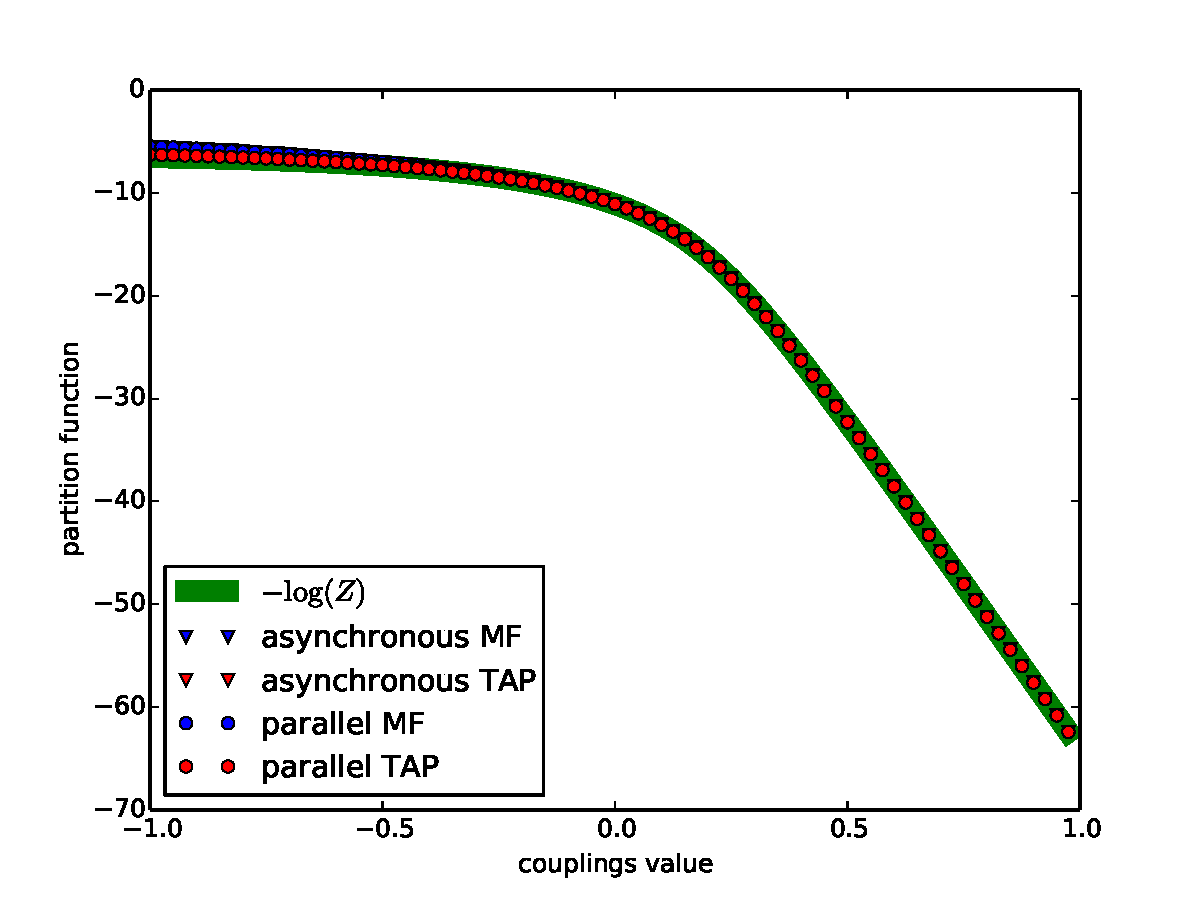
\includegraphics[width=\linewidth]{../../../Code/DRBM/toy/sameCouplingsRBMZ}
\label{fig:drbm}
  \caption[1]{DRBM TAP2 TAP3 PCD}
\end{figure}

The average squared errors on training and validation data sets (Figure \ref{mse}) confirms the visual assessment of reconstructions. The mean field obtains the highest score while TAP2 and TAP3's scores are slightly higher then with training DBN using PCD approach. 

\begin{figure}[!htb]
 %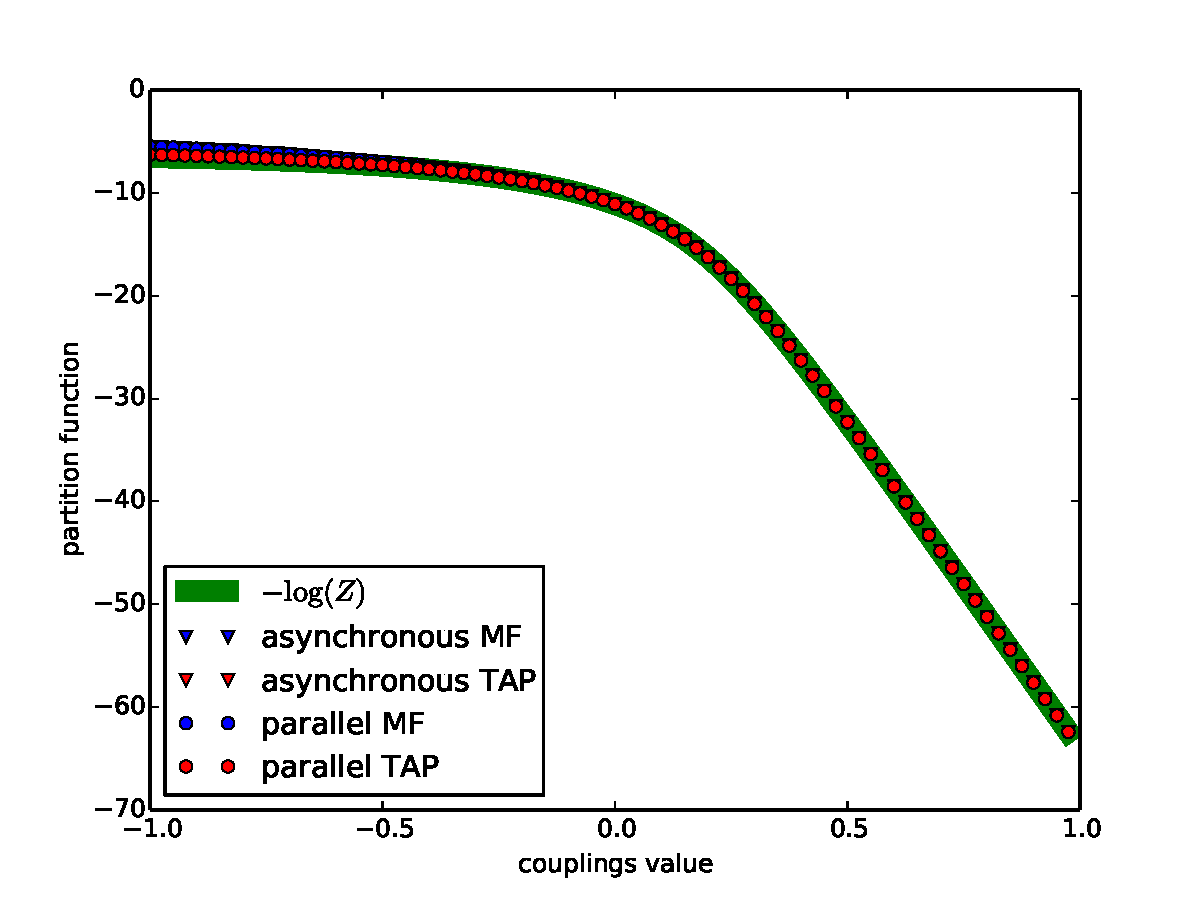
\includegraphics[width=\linewidth]{../../../Code/DRBM/toy/sameCouplingsRBMZ}
\label{fig:mse}
  \caption[1]{shows the mean squared error on training and validation data sets for different methods for pre-training the RBMs.}
\end{figure}

TAP2 0.0515471685931
MF 0.0610472665952
TAP3 0.0511828595047
PCD 0.048851695881

Those results confirms the observations from the previous chapter and shows that additional higher-order approximations substantially improves the quality of learned magnetizations which in turns helps learning a better model.

\end{document}


\subsection{Semi RBM}
SEE IF IT IS WORTH IT.
\subsubsection{Exploiting the SRBM structure}
Clamped free energy can be written in the form:
\begin{align}
\begin{split}
\mathcal{F}^c(\mathbf{v}) = & \sum_\mathbf{h} e^{-E(\mathbf{v}, \mathbf{h})} = e^{\mathbf{b}'\mathbf{v}}\sum_{h_1}...\sum_{h_m}e^{-E(\mathbf{v}, \mathbf{h})} \\
=&  e^{\mathbf{b}'\mathbf{v}} \sum_{h_1} e^{h_1 (c_1 + W_{1\bullet}\mathbf{v})}... \sum_{h_m} e^{h_m (c_m + W_{m\bullet}\mathbf{v})} \\
= & e^{\mathbf{b}'\mathbf{v}} \prod_{j=1}^{m} \left( 1 + e^{c_i + W_{i\bullet}\mathbf{v}} \right)
\label{eq:freeEnergy}
\end{split}
\end{align}